\documentclass[Ex4_Zusammenfassung.tex]{subfiles}

\begin{document}

\section{Angeregte Zustände in Atomkernen}
\textbf{von \hein \& \martina}\\

\subsection*{Rückblick}
Bei 2--atomigen Molekülen sind verschiedene Formen der Anregung möglich. Die niedrigsten angeregten Zustände sind Rotationen, außerdem sind auch Vibrationen möglich. Vibrationsanregungen haben deutlich höhere Energien als Rotationsanregungen: $E_{\text{Vib}}  \simeq 100\cdot E_{\text{Rot}}$

\subsection{Angeregte Zustände}
Kerne mit abgeschlossenen Schalen sind kugelsymmetrisch. In der Nähe abgeschlossener Schalen wird ein Kern immer noch am besten durch das Schalenmodell beschrieben. Ist die Schale nicht abgeschlossen, ist der Kern nicht mehr kugelsymmetrisch, sondern ähnelt einem Ellipsoid. 
\begin{figure}[h]
	\begin{subfigure}[t]{0.3\textwidth}
		\centering
		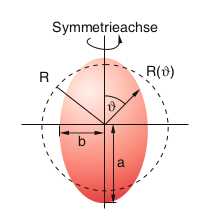
\includegraphics[scale=0.55, trim= 0 -0.45cm 0 0]{ellipsoid_1.png}
	\end{subfigure}
	~
	\begin{subfigure}[b]{0.7\textwidth}
		\centering
		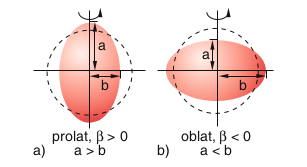
\includegraphics[scale=0.6]{ellipsoid_2.png}
	\end{subfigure}
	\caption{Allgemeine Beschreibung der Ellipsoiden (links), und die Bezeichnungen für die 2 verschiedenen Formen (rechts, a und b)}
	\label{ellipsoids}
\end{figure}
Ein rotationssymmetrischer Ellipsoid kann durch Polardarstellung dargestellt werden:
\begin{align}
	R(\vartheta) &= R_0 \left[ 1 + \beta \cdot Y_2^0 (\cos \vartheta ) \right], \quad \beta \ll 1\\
	R_k &= R_0 \cdot \left[ 1 + \sqrt{\frac{5}{4\pi}} \beta \cos\lp \vartheta - \frac{2 \pi k}{3}\rp  \right]
\end{align}
wobei $\beta$ einen Deformationsparameter darstellt. 

Dabei treten zwei Formen auf: Oblaten und Prolaten (Abb. \ref{ellipsoids} rechts). 

\subsection{Rotation}
Da in den Kernspektren äquidistante Linien auftauchen, schließt man nun auf Rotationsanregungen. Durch Stöße mit schweren Projektilen (Protonen, $\alpha$--Teilchen) können Drehimpulse erzeugt und der Kern damit zu Rotation angeregt werden. Da auf kugelsymmetrische Objekte kein Drehimpuls übertragen werden kann, werden die Kerne als deformiert angenommen. 
\begin{figure}[h]
	\centering
	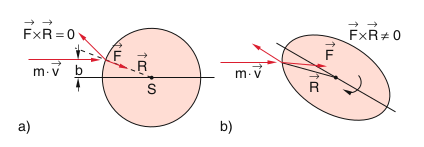
\includegraphics[scale=0.4]{deformiert.png}
	\caption{Kein Drehimpulsübertrag bei kugelsymmetrischem Kern (a), Drehimpulsübertrag auf deformierten Kern (b).}
\end{figure}
Entsprechend steht die Rotationsachse immer senkrecht auf der Symmetrieachse, da sonst wie bei der Kugel kein Drehmoment wirken kann. 

Die Energieniveaus eines quantenmechanischen Rotators sind
\begin{equation}
	E = \frac{\hslash^2}{2 \Theta} I (I+1)
\end{equation}
wobei $\Theta$ das Trägheitsmoment und $I$ die Drehimpulsquantenzahl des Kerns darstellen. 

Aus den Abständen zwischen zwei Spektrallinien lässt sich $\Theta$ ermitteln. Aufgrund der Paritätserhaltung sind nur gerade Werte für $I$ erlaubt:
\begin{align}
	\intertext{hierfür sei} A = \frac{\hslash^2}{2 \Theta}
	\intertext{und somit folgt}
	\Delta E = E_I - E_{I-2} &= AI(I+1) - A(I-2)(I-1)\\
	&= A(I^2 + I - I^2 + 3I - 2)\\
	&= A(4I - 2)\\
	&= 4AI - 2A
\end{align}
$\Delta E$ entspricht einer Spektrallinie. Also folgt für die Differenz zweier Spektrallinien:
\begin{align}
	\Delta (\Delta E) &= 4A(I+2) -2A - 4AI + 2A\\
	&= 4AI + 8A - 4AI \\
	&= 8A = 8 \frac{\hslash^2}{2\Theta}
\end{align}
Die berechneten $\Theta$ sind um den Faktor 2 zu groß, da man den Kern nicht als starren Rotator annehmen kann. 
\subsection{Vibration}
kann auch bei kugelsymmetrischen Kernen auftreten. Dabei gibt es 2 wesentliche Schwingungstypen:
\begin{itemize}
	\item Radiale Kompressionssschwingung:\\
	Die Dichte des Kerns ändert sich periodisch und es tritt kein Drehimpuls auf. Da die Kernmaterie aber fast inkompressibel ist, muss die Anregungsenergie hierfür sehr groß sein.
	\item Oberflächenschwingung:\\
	Das Kernvolumen ändert sich nicht, aber der Kern wird deformiert. Hier kann z.B. die Kugel abwechselnd in Oblate und Prolate übergehen.
\end{itemize}
Abhängig von der Art der Schwingung erhält man bei genügend kleinen Amplituden die Energiewerte des harmonischen Oszillators:
\begin{equation}
	E_{\text{Vib}} = \hslash \omega_{\ell, m} \lp n + \frac{1}{2} \rp
\end{equation}
$\omega_{\ell, m}$ hängt von der Art der Schwingung und Deformation ab.

\section{Schalenmodell}
Wie kann man die Peaks in Abb. \ref{kernbindungsenergie} und die Zahlen der stabilen Isotope erklären? Der Kern weißt Schalenverhalten auf, ähnlich wie Elektronen in der Hülle. 

Als Näherung des Kernpotentials betrachten wir das Wood--Saxon Potential:
\begin{equation}
	V(r) = - \frac{V_0}{1+ \exp \lp \frac{r-R}{a} \rp }
\end{equation}
wobei $V_0$ die Potentialtopftiefe, $a$ die Oberflächendicke eines Kerns und $R = r_0 A^{\nicefrac{1}{3}}$ der Kernradius mit $r_0= \SI{1.25}{fm}$ und Massenzahl $A$ sind. 

Wir nehmen hierbei an, dass die Kräfteverteilung $\propto$ Dichte $\propto$ Ladungsverteilung $\propto$ Fermiverteilung ist.
\begin{figure}[h]
	\centering
	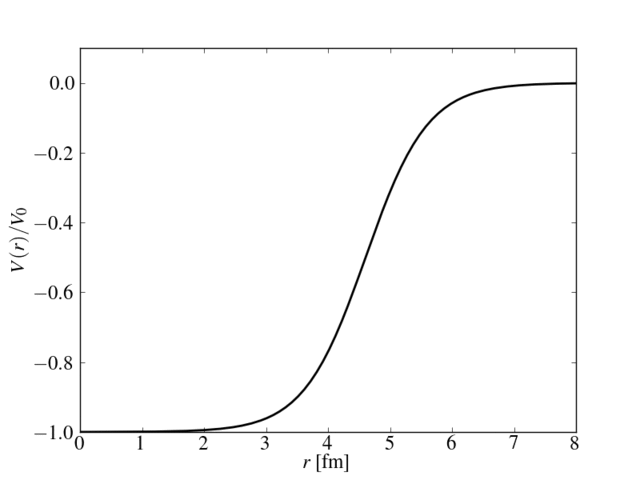
\includegraphics[scale=0.4]{woodsaxon.png}
	\caption{Wood--Saxon--Potential mit $A=50$ und $a=\SI{0.5}{fm}$}
\end{figure}

Wir versuchen die Schrödinger Gleichung zu lösen, um konkrete Energiezustände fur Schalen zu erhalten. \Lightning Problem: $\nexists$ analytische Lösung für Wood--Saxon. Daher nähern wir das Wood--Saxon Potential durch einen harmonischen Oszillator oder durch ein Kastenpotential. Die Lösung der Schrödinger--Gleichung ergibt:
\begin{equation}
	 E_N = \hslash \omega \lp N + \frac{3}{2} \rp - V_0
\end{equation}
wobei $N = 2(n-1) + \ell $ mit der Bahndrehimpulsquantenzahl $\ell$ und $\ell$ die Werte $N,\ N-2,\ ...\ 1 \text{ oder } 0$ annimmt. $n$ ist die Anzahl der radialen Knoten.

Für die Entartung $g(N)$ ergibt sich
\begin{equation}
	g(N) = \frac{1}{2} (N+1)(N+2)
\end{equation} 

Wir betrachten die Schalen:
\begin{table}
	\centering
	$
	\begin{array}{llclccc}
	n & \ell & N & \text{Orbitale } n\ell & \text{Parität} & \text{Entartungsgrad } 2g(N) & \sum 2g(N) \\ \hline
	1 & 0 & 0 & 1s & + & 2 & 2 \\ 
	1 & 1 & 1 & 1p & - & 6 & 8 \\ 
	1,\ 2 & 2,\ 0 & 2 & 2s,\ 1d & + & 12 & 20 \\ 
	1,\ 2 & 3,\ 1 & 3 & 2p,\ 1f & - & 20 & 40 \\ 
	1,\ 2,\ 3 & 4,\ 2,\ 0 & 4 & 3p,\ 2d,\ 1g & + & 30 & 70
	\end{array} 
	$
	\caption{Der Faktor 2 in der Spalte der Entartung rührt daher, dass der Spin auch entartet ist. }
\end{table}
Diese Zahlen ähneln den Elektronenschalenzahlen. Aber experimentell stellen wir die magischen Zahlen (2, 8, 20, 28, 50, 82, ...) als besonders stabil fest (woraus folgt, dass dort Schalen sein müssen!) 

Bisher haben wir die Entartung durch den Spin nicht betrachtet. Die Spin--Bahn--Kopplung liefert weitere Aufspaltung der Energie--Niveaus. Wir betrachten den Gesamtdrehimpuls
\begin{equation*}
	\vec{j} = \vec{\ell} + \vec{s} 
\end{equation*}
um die Differenz der neuen Energieaufspaltungen zu erhalten:
\begin{equation}
	E_{\ell s} = c_{\ell s} \vec{\ell} \cdot \vec{s} 
\end{equation}
wobei hier 
\begin{align*}
	\vec{\ell} \cdot \vec{s} &= \frac{1}{2} \lp \pvec{j}^2 - \pvec{\ell}^2 - \pvec{s}^2 \rp
	\intertext{was auf den Zustand angewendet folgendes ergibt:}
	&= \frac{1}{2} \hslash^2 \lp j(j+1) - \ell(\ell + 1) - s(s+1) \rp 
\end{align*}
Außerdem ist hier $s=\nicefrac{1}{2}$ (Nukleonen und Fermionen) und $j=\ell \pm \nicefrac{1}{2}$.
\begin{equation}
	\vec{\ell} \cdot \vec{s} = 
		\begin{cases}
			\frac{1}{2} \hslash^2 \ell & j=\ell + \frac{1}{2}\\
			-\frac{1}{2} \hslash (\ell + 1) & j=\ell - \frac{1}{2}
		\end{cases}
\end{equation}
Das Niveau $j=\ell + \nicefrac{1}{2}$ ist offenbar energetisch günstiger. Außerdem sieht man, dass die Energieaufspaltung
\begin{equation}
	\Delta E|{\ell s} = \lp \ell + \frac{1}{2} \rp \hslash^2 c_{\ell s} 
\end{equation}
mit zunehmendem $\ell$ größer wird. Dies führt zu sehr starker Überlappung der ursprünglichen Schalen (Abb. \ref{schalen}).
\begin{figure}[h]
	\centering
	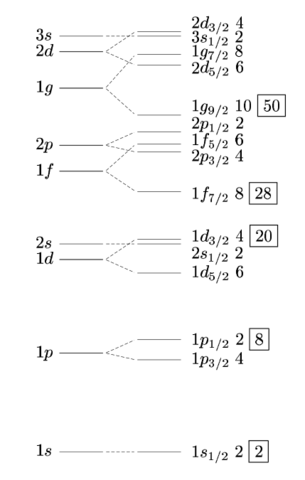
\includegraphics[scale=0.5]{schalenmodell.png}
	\caption{$(n \ell) \longrightarrow (n\ell_j)$}
	\label{schalen}
\end{figure}

Die nun entstehenden Energieniveaus entsprechen den magischen Zahlen. Offenbar liegt also im wesentlichen Unterschied vom Schalenmodell der Elektronen in den Hüllen hier ein eine viel stärkere Spin--Bahn--Kopplung vor. 
\end{document}